% Presupposition CogSci 2016

In this section we introduce an extension to Rational Speech-Act (RSA) model
\cite{FrankGoodman2012:Predicting-Pragmatic-Reasoning-,GoodmanStuhlmuller2013:Knowledge-and-I} 
to account for the projection phenomenon of change-of-state verbs under negation,
 by formalizing the ideas introduced in the previous section. 
We will continue to use our working example of the conversation between Alice and Bob
 regarding John's smoking habit.

We consider the following relevant utterances: ``John smokes,'' 
 ``John smoked,'' ``John has always smoked,''
 ``John stopped smoking,'' ``John started smoking,'' 
 ``John has never smoked,'' and their negations. 
In addition, we introduce the null utterance ``'' (say nothing).
The prior probability of an utterance depends on the number of content words 
 (i.e., negation and auxiliaries are excluded) that it has.
The shorter an utterance, the higher its prior probability is, as defined in 
 (\ref{eq:utterance-prior}).

\vspace{-6pt}
\begin{equation}
\Pr(u) \propto 2^{-\#\textrm{content-words}(u)}\label{eq:utterance-prior}
\end{equation}

The meaning/denotation of an utterance is standardly defined as the set of worlds 
 where the utterance is true.
We define a world $w$ as a pair.
Its first element is whether John smoked in the past 
 and its second element is whether John smokes now. 
This gives us a set of four possible worlds (the \emph{universe} 
 $U=\{(T, T), (T, F), (F, T), (F, F)\}$).
All positive utterances and their denotations are listed in Table~\ref{tab:pos-utt-denotations}.
In addition, we define that saying nothing is always true, and that the denotation 
 of the negation of an utterance $u$ is $U-\intp{$u$}$.
%``John stopped smoking'' is true iff 
% John smoked in the past and does not smoke now, i.e., $\intp{John stopped smoking}$
% $=\{\verb+(#t #f)+\}$, and we have 
%$\intp{John didn't stop smoking}= U - \{\verb+(#t #f)+\} = \{\verb+(#t #t)+,
% \verb+(#f #t)+, \verb+(#f #f)+\}$. 

\begin{table}
\centering
\begin{tabular}{cc}
$u$ &  $\intp{$u$}$  \\ \hline
``John smokes''  & $\{(T, T), (F, T)\}$ \\ 
``John smoked'' & $\{(T, T), (T, F)\}$ \\ 
``John has always smoked'' & $\{(T, T)\}$ \\
``John stopped smoking'' & $\{(T, F)\}$ \\
``John started smoking'' & $\{(F, T)\}$ \\
``John has never smoked'' & $\{(F, F)\}$ \\ \hline
\end{tabular}
\vspace{-1ex}
\caption{Positive utterances and their denotations \label{tab:pos-utt-denotations}}
\vspace{-3ex}
\end{table}


A \emph{Question Under Discussion} (QUD) is a function $Q$ that takes a possible world as 
 its argument and returns the answer to the question in this world.
For example, QUD$_\textrm{now}$ is the question ``Does John smoke now?'' 
It takes a world and returns its second element, which answers whether 
 John smokes now. 
Another example is the maximal QUD$_\textrm{max}$, which is the identity function. 
Intuitively, QUD$_\textrm{max}$ is asking which is the current world.
It is maximal in the sense that knowing its answer means knowing the answer to 
 any QUD.
 
To account for projective behavior, we propose 
 additional components and assumptions to the standard RSA model in the literature
 \cite{FrankGoodman2012:Predicting-Pragmatic-Reasoning-,GoodmanStuhlmuller2013:Knowledge-and-I,GoodmanLassiter2015-Chapter}.
To better illustrate why each of them is necessary and how they contribute to 
 the model's prediction, we will present the model incrementally. 
We will start with the standard RSA model, point out its problems, motivate 
 a modification, explain the problem it addresses, review the remaining issues, 
 motivate another modification, and so on, until we reach the final model.

\ 

\noindent\textbf{Standard RSA model}

In the standard RSA model (augmented with QUD as in \citeA{GoodmanLassiter2015-Chapter}), the literal listener, given an utterance and a QUD, 
 randomly samples a world that is consistent with the utterance, 
 and returns the value of the QUD in that world, as in (\ref{eq:literal-noCG}). 
In this paper we always assume that all worlds are equally likely \emph{a priori}, 
 i.e. $\Pr(w)=1/4$ for each $w$.

\vspace{-6pt}
\begin{equation}
L_0(Q(w) \mid u, Q) \propto  \sum_{w'\in \intp{u}} \delta_{Q(w)=Q(w')} \cdot \Pr(w')  \label{eq:literal-noCG}
\end{equation}

% \ndg{this notation isn't the best: the distribution over Q(w) isn't fully defined and the impact of literal meaning is better specified by a delta function.
% it's cleaner to handle the QUD in the speaker.i'd do it like: 
% $P_{L_0}(w \mid u) \propto \delta_{w\in \intp{u}}$ 
% and $P_{S}(u\mid w,Q) \propto P(u)\sum_{Q(w)=Q(w')}P_{L_0}(w' \mid u)$.
% i'm not going to make this change, since it affects a lot. y'all can if you want, or we can do it in the post-submit revision...}
 
\begin{table*}
\centering
\begin{tabular}{c|c|c|c|c}
         & Standard (no CG + QUD$_\text{max}$ ) & Uniform CS + QUD$_\text{max}$ & CG prior + QUD$_\text{max}$ & CG prior + QUD$_\text{now}$ \\ \hline 
literal  & $L_0(Q(w) \mid u, Q) \propto  \sum_{w'\in \intp{u}} \delta_{Q(w)=Q(w')} \cdot \Pr(w') $ & 
\multicolumn{3}{c}{$L_0(Q(w) \mid u, C, Q) \propto  \sum_{w'\in C\cap \intp{u}} \delta_{Q(w)=Q(w')} \cdot \Pr(w')$} \\
speaker  & $S(u | w, Q) \propto \Pr(u) \cdot L_0(Q(w) \mid u, Q)^\alpha $ & \multicolumn{3}{c}{$S(u | w, C, Q) \propto \Pr(u) \cdot L_0(Q(w) \mid u, C, Q)^\alpha$} \\
listener & $L(w \mid u, Q) \propto \Pr(w) \cdot S(u \mid w, Q)$ & \multicolumn{3}{c}{$L(w, C \mid u, Q) \propto \Pr(w) \cdot \Pr(C) \cdot S(u \mid w, C, Q)$} \\
CG prior & -- & $\Pr(C) \propto 1$ & \multicolumn{2}{c}{$\Pr(C) \propto \sum_{CG\subseteq\text{Obs}} P(CG) \cdot \delta_{C=\cap CG}$}\\
%\Pr(C)=0.95\cdot\Pr(C=\cap\text{CG}_\text{Obs})+0.05\cdot 1/15$} \\
QUD      & $\text{QUD}_\text{max}(w)=w$ & $\text{QUD}_\text{max}(w)=w$ & $\text{QUD}_\text{max}(w)=w$ & $\text{QUD}_\text{now}((x,y))=y$\\
%QUD      & \multicolumn{3}{c}{$\text{QUD}_\text{max}(w)=w$} & $\text{QUD}_\text{now}((x,y))=y$\\
\hline
\end{tabular}
\caption{Specifications of four RSA models \label{tab:models}, with $\Pr(w)\propto1$ and $\Pr(u) \propto 2^{-\#\textrm{content-words}(u)}$ for all four models}
\vspace{-2ex}
\end{table*} 
 
\begin{figure*}
 \centering
 \subfigure[No CG + QUD$_\text{max}$]{\label{fig:vanillaRSA}
 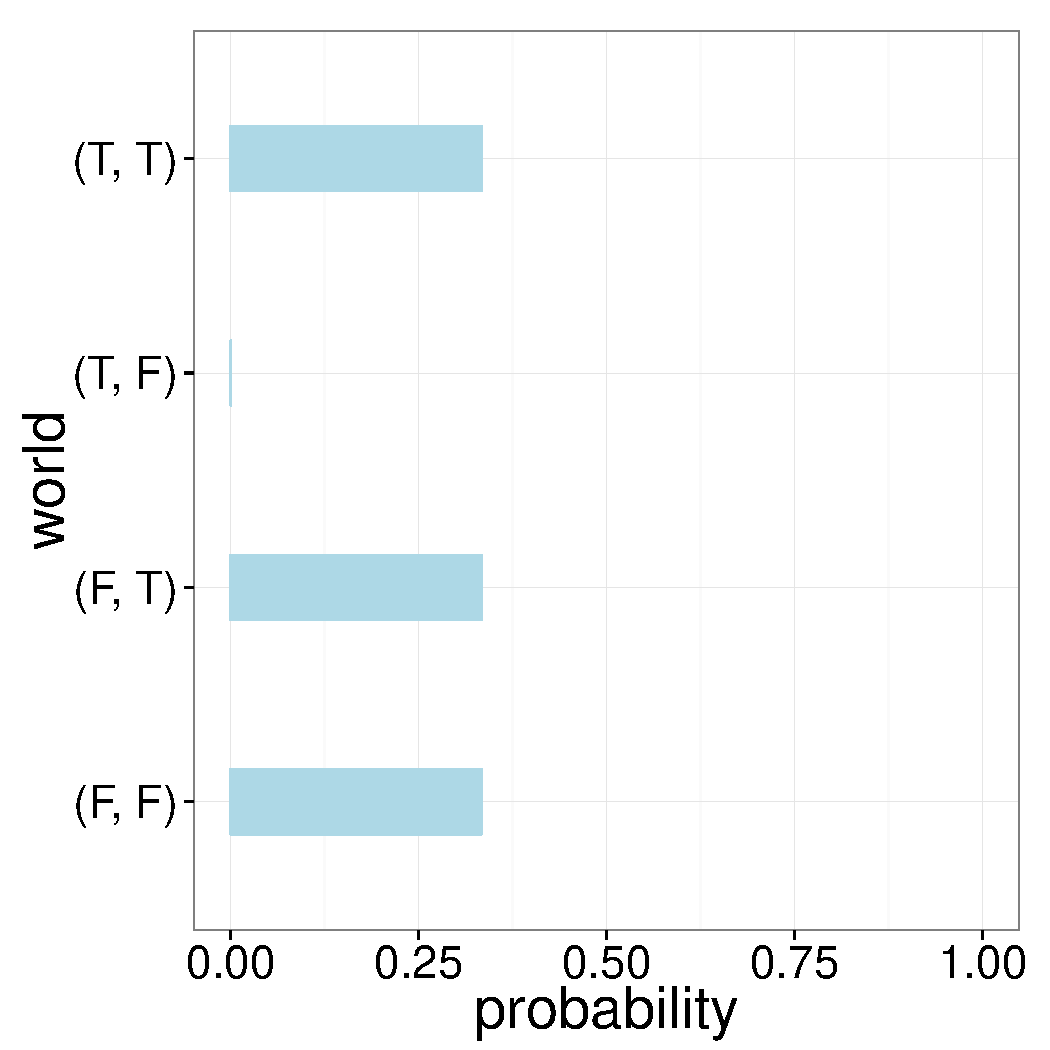
\includegraphics[scale=0.23]{figs/vanillaRSA.pdf}}
 \subfigure[Uniform CS + QUD$_\text{max}$]{\label{fig:RSA_uniformCG}
 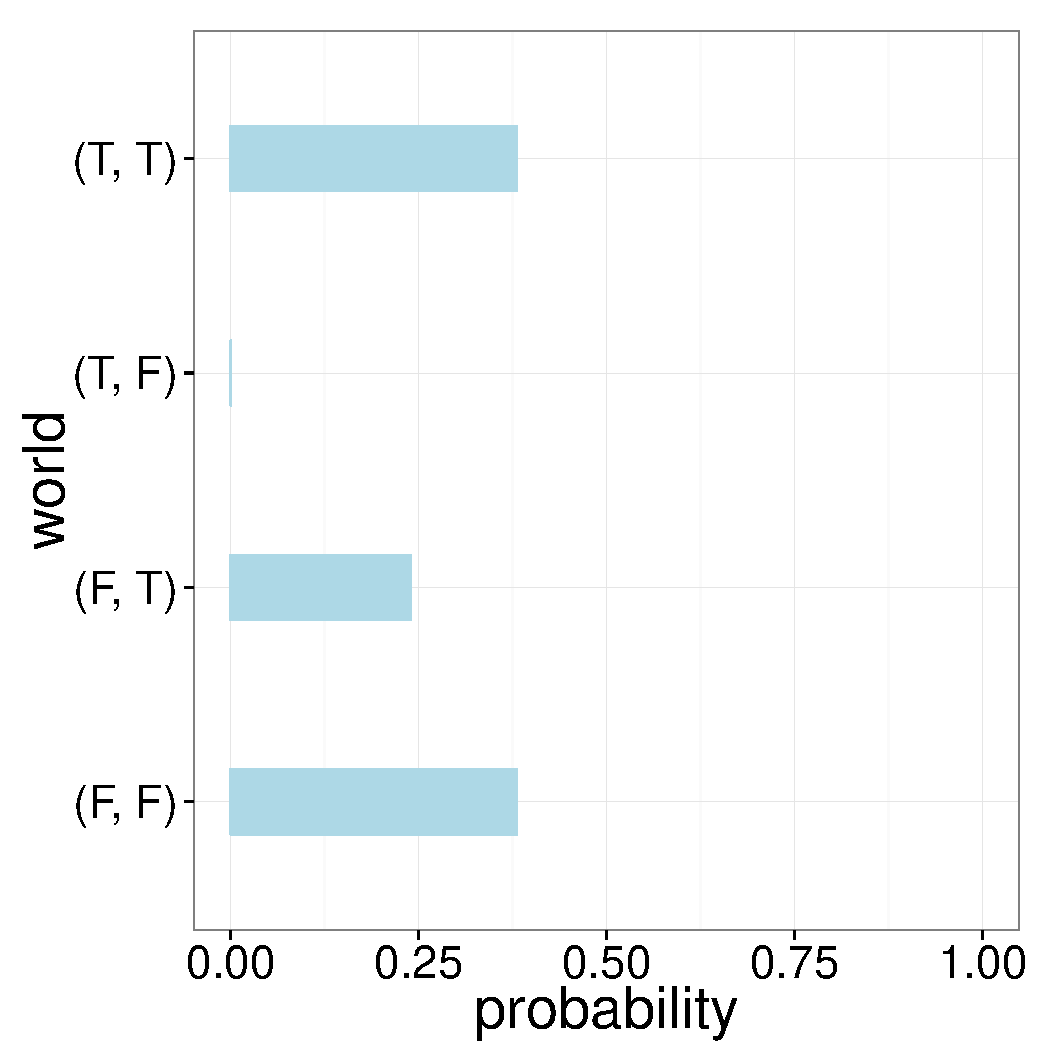
\includegraphics[scale=0.23]{figs/uniformCG.pdf}}
 \subfigure[CG prior + QUD$_\text{max}$]{\label{fig:RSA_CGprior}
   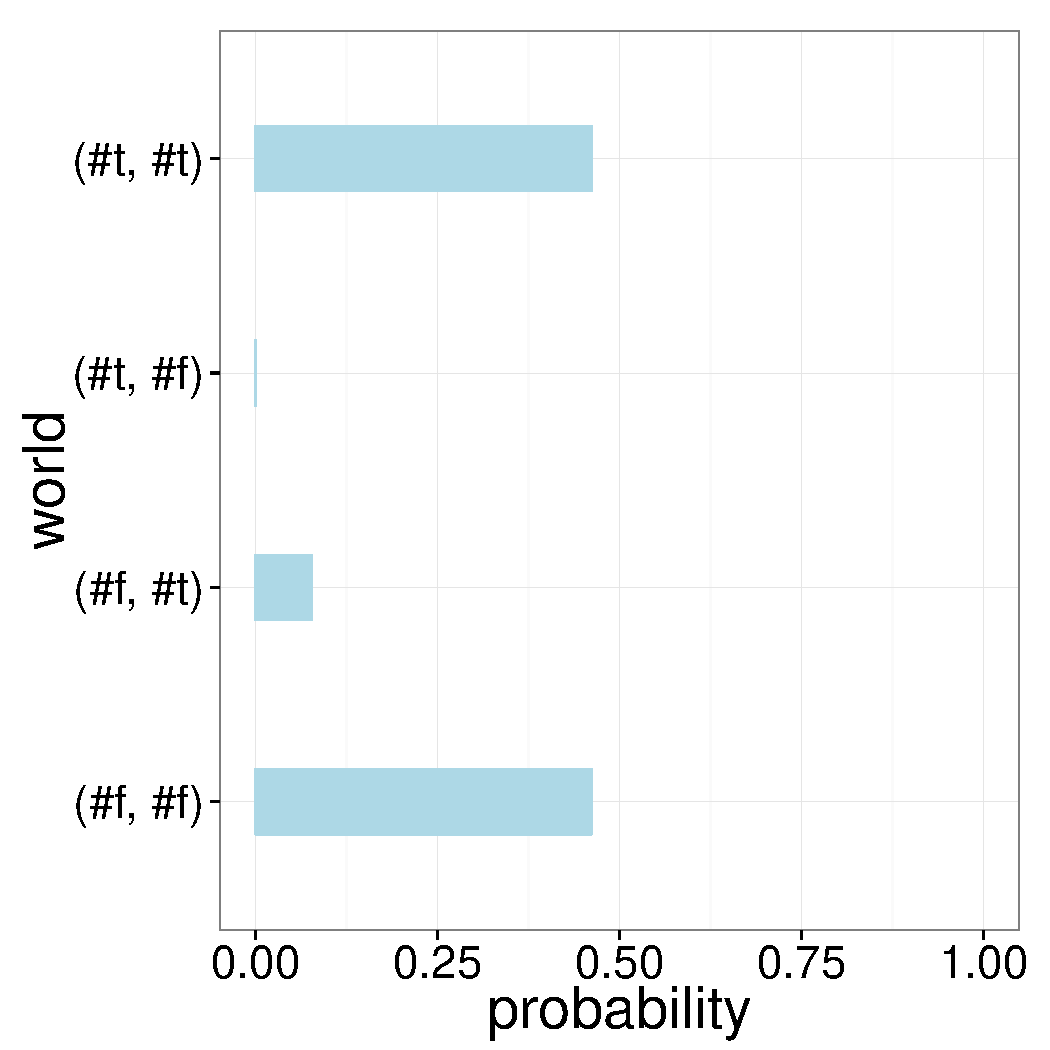
\includegraphics[scale=0.23]{figs/CGprior.pdf}}
 \subfigure[CG prior + QUD$_\text{now}$]{\label{fig:RSA_QUDnow}
   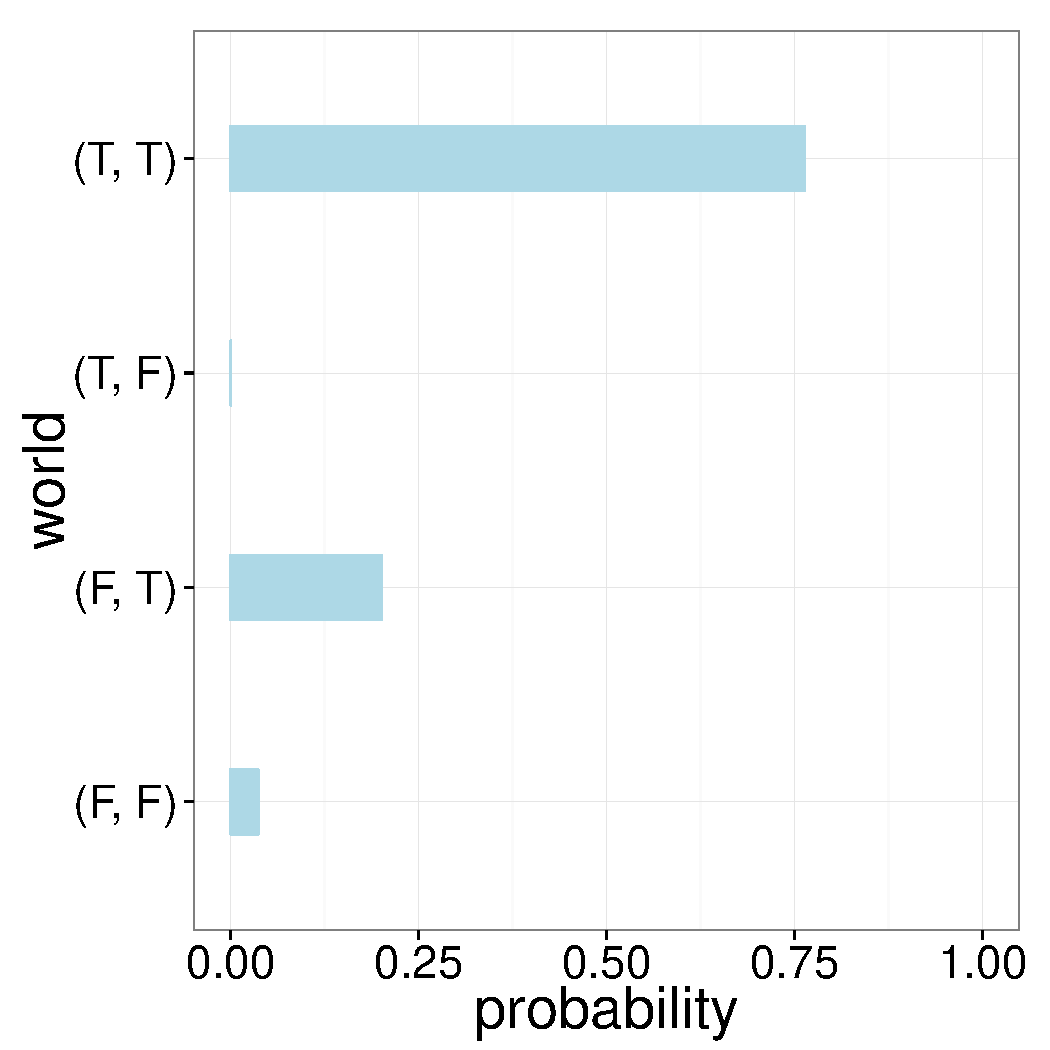
\includegraphics[scale=0.23]{figs/QUDnow.pdf}}
 \caption{Pragmatic listener after hearing ``John did not stop smoking'' for each model, with $\alpha=6$ }
\end{figure*}

Here $\delta$ subscripted with a statement is defined to be $1$ if the statement 
 is true and $0$ otherwise.
%(\ref{eq:literal-noCG}) specifies a distribution over possible answers to the QUD.
For example, if $Q$ is QUD$_\textrm{max}$, which asks for a complete specification of the state of the world, after hearing "John didn't stop smoking," the literal listener will rule out world $(T, F)$, and return the remaining 3 worlds with equal probability.


Given the actual world and the QUD, the probability of 
 the speaker's utterance $u$ depends on two factors: the utterance prior 
 and the probability that the utterance will make the literal listener 
 return the correct answer to the QUD, as in (\ref{eq:speaker-noCG}).

\vspace{-6pt} 
\begin{equation}
S(u | w, Q) \propto \Pr(u) \cdot L_0(Q(w) \mid u, Q)^\alpha 
\label{eq:speaker-noCG}
\end{equation}

Here $\alpha$ is a rationality parameter controlling the extent to which 
 the speaker optimizes her utterance to induce the correct answer from the 
 literal listener. 
When $\alpha \rightarrow \infty$, the speaker will choose utterances that 
 strictly maximize the probability of inducing the right answer.
In this paper we set $\alpha=6$, but the qualitative predictions do not hinge on 
 this specific value.

The pragmatic listener, given the QUD, infers the actual world given the speaker's utterance, using Bayes' rule (\ref{eq:listener-noCG}).

\vspace{-6pt} 
\begin{equation}
L(w \mid u, Q) \propto \Pr(w) \cdot S(u \mid w, Q) \label{eq:listener-noCG}
\end{equation}

The standard RSA model is summarized in the first column of Table~\ref{tab:models},
 and the predicted pragmatic listener's distribution over worlds is shown in Figure~\ref{fig:vanillaRSA}.
As we can see, the standard RSA model predicts a uniform distribution over the
 three worlds that are consistent with the literal meaning of 
 ``John did not stop smoking''. It therefore fails to capture the projective content --- the inference that  
 John used to smoke.

The reason for this failure is that ``John did not stop smoking'' is equally
 under-informative in any of the three worlds compatible with its literal meaning.
For example, suppose the actual world is $(T, T)$. Since the 
 literal listener will return this world with probability only $1/3$ after hearing ``John did not stop smoking,'' the speaker is unlikely to choose this utterance.
She is more likely to say ``John has always smoked'' instead, which will always
 induce the correct answer. 
The same holds for the other two worlds $(F, T)$ and $(F,
 F)$ and therefore the pragmatic listener in the standard RSA model will 
 infer that the three worlds are equally likely.
 
\ 

\noindent\textbf{RSA with common ground}

\begin{figure*}
 \centering
 \subfigure[Uniform CS + QUD$_\text{max}$]{\label{fig:joint-uniform}
  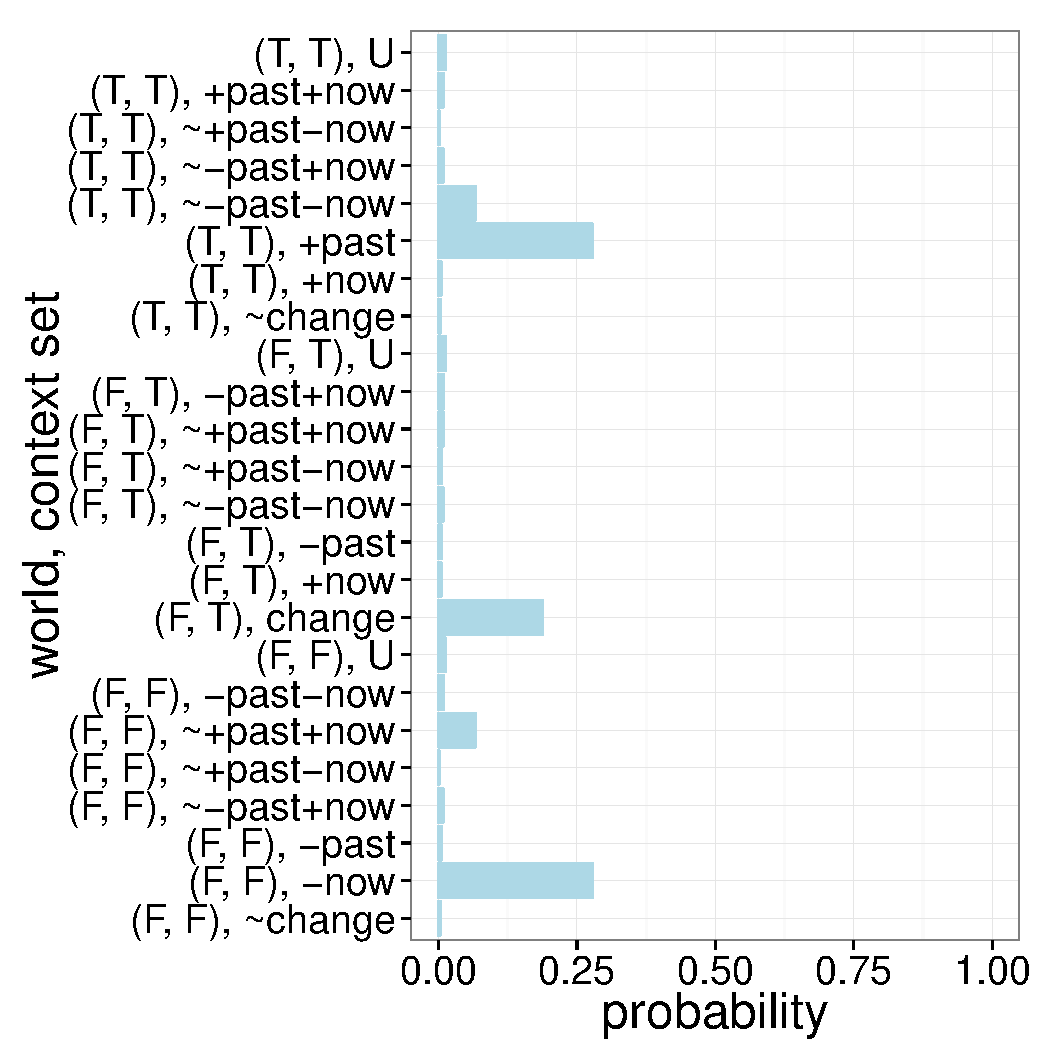
\includegraphics[scale=0.48]{figs/joint_uniformCG_QUDmax.pdf}} 
  \hspace{5pt}
 \subfigure[CG prior + QUD$_\text{max}$]{\label{fig:joint-CGprior}
 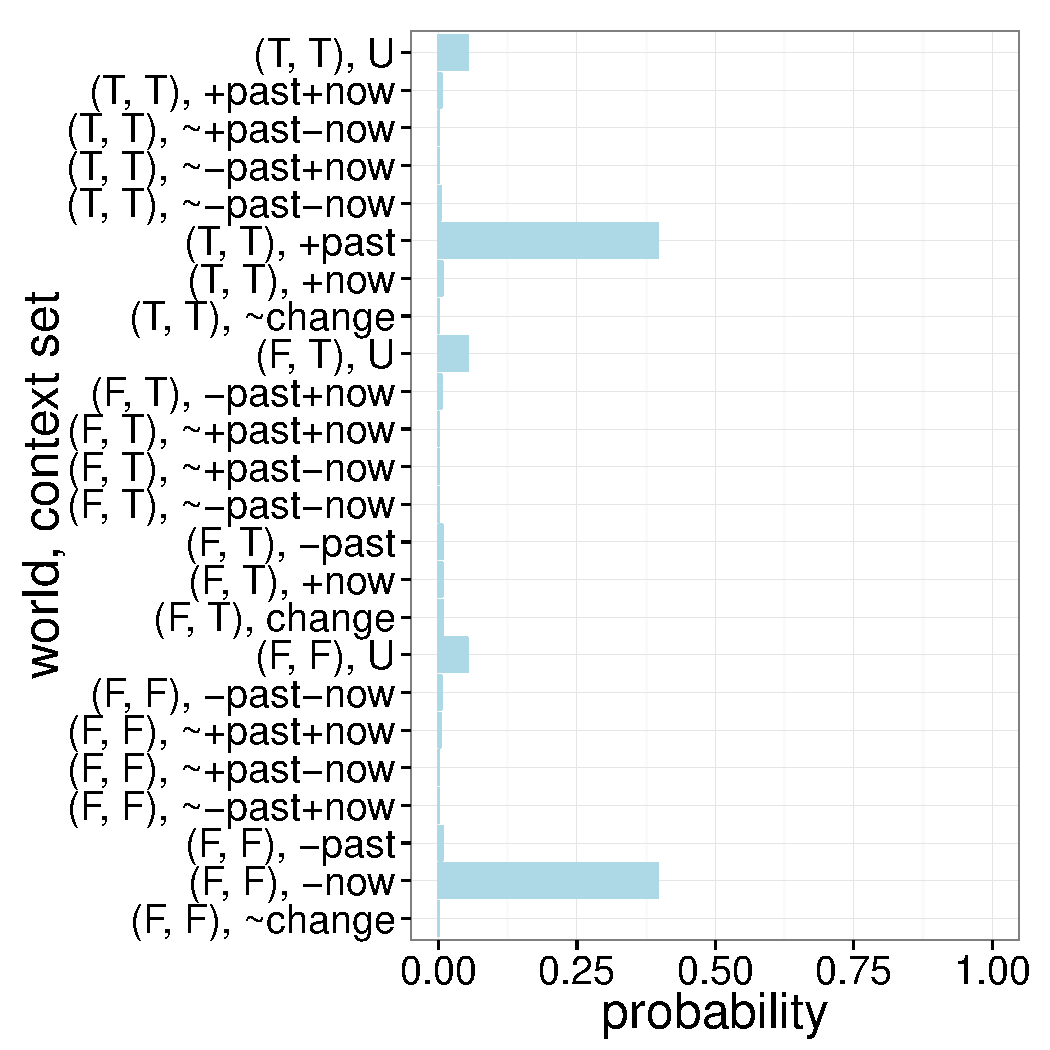
\includegraphics[scale=0.48]{figs/joint_CGprior_QUDmax.pdf}} 
% \hspace{5pt}
%  \subfigure[CG prior + QUD$_\text{now}$]{\label{fig:joint-QUDnow}
%  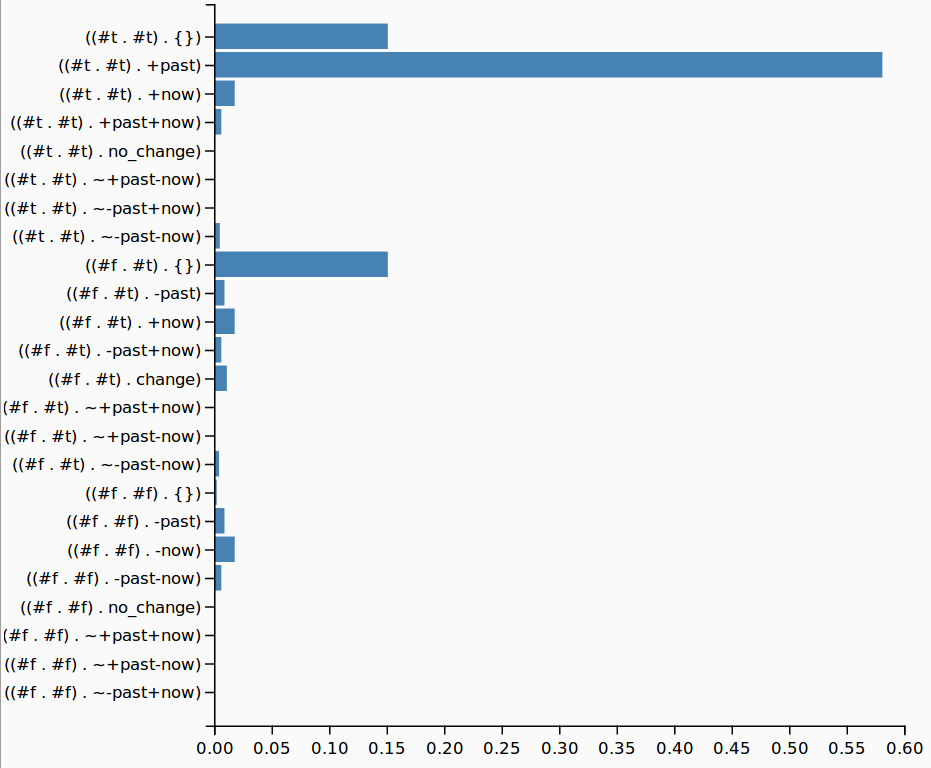
\includegraphics[scale=0.26]{figs/alpha6CGprior_QUDnow.png}}%alpha6cost1eqllhcg
 \caption{Pragmatic listener after hearing ``John did not stop smoking,'' with $\alpha=6$\label{fig:prior}}
\end{figure*}

We have seen that one important reason that the standard RSA model fails to 
 capture the projective content of ``John did not stop smoking'' is that its literal
 meaning is under-informative when considered in the entire universe $U$.
However, as discussed before, there can be information taken for granted by the
 speaker and the listener, i.e., the common ground, 
and an utterance that is under-informative when considered in the entire universe $U$ may 
 nevertheless be informative when evaluated in the common ground.
To formalize this observation, we now add common ground to the RSA model.

We first define a related notion. 
A \emph{context set} $C$ is a non-empty subset of the universe \cite{Stalnaker1974:Pragmatic-Presuppositions}.
Since we have 4 possible worlds, there are $2^4-1=15$ different context sets.
These context sets are intuitively named. 
For example, \verb=+past= is the context set
 that contains $(T, T)$ and $(T, F)$,
\verb=+past+now= contains only $(T, T)$,
$\sim$\verb=+past+now= contains all the worlds except $(T, T)$ ($\sim A$ is defined to be $U-A$, i.e., $A$'s complement), 
and \verb=change= is the context set that contains $(T, F)$ 
 and $(F, T)$.

A literal listener, given an utterance, the current context set and QUD, 
 randomly samples a world that is consistent with both the utterance and 
 the context set, and returns the value of the QUD in that world, as in  
 (\ref{eq:literal-CG}).

\vspace{-6pt}
\begin{equation}
L_0(Q(w) \mid u, C, Q) \propto  \sum_{w'\in C\cap \intp{u}} \delta_{Q(w)=Q(w')} \cdot \Pr(w') \label{eq:literal-CG}
\end{equation}

For example, given context set \verb=+past= and QUD$_\text{max}$, 
 after hearing ``John did not stop smoking,'' the literal listener will rule out 
 $(T, F)$ because of the utterance's literal meaning, and 
 $(F, T)$ and $(F, F)$ because 
 they are incompatible with the context set.
Therefore he will always return $(T, T)$.
We can see from this example that an utterance that is under-informative 
 when the entire universe is considered can be informative in some other 
 context sets.

The new speaker model is almost the same as (\ref{eq:speaker-noCG}), except that 
 it is relativized to the current context set, as in (\ref{eq:speaker-CG}).

\vspace{-6pt}
\begin{equation}
S(u | w, C, Q) \propto \Pr(u) \cdot L_0(Q(w) \mid u, C, Q)^\alpha \label{eq:speaker-CG}
\end{equation}
 
Finally, given an utterance and the QUD, the pragmatic listener now jointly infers 
 the real world and the context set the speaker assumes when she produces the utterance. 

\vspace{-6pt} 
\begin{equation}
L(w, C \mid u, Q) \propto \Pr(w) \cdot \Pr(C) \cdot S(u \mid w, C, Q)
\label{eq:listener-CG}
\end{equation}

We need to specify a prior distribution $\Pr(C)$ 
 over context sets in (\ref{eq:listener-CG}).
We consider two possibilities. 
First, we consider a uniform distribution over all context sets, i.e., 
 $\Pr(C)\propto 1$.
Assuming the maximal QUD, the model is summarized in the second column of 
 Table~\ref{tab:models} and the pragmatic listener's marginal distribution over 
 worlds is shown in Figure~\ref{fig:RSA_uniformCG}.
We can see that this model predicts that $(F, T)$ is slightly 
 less likely than $(T, T)$ and $(F, F)$, 
 and $(T, T)$ has the same probability as $(F, F)$. 
This does not capture projection.


% explanation of why a uniform prior is undesirable
%
%
%Clearly this model does not capture projective phenomena, either. 
%But let us take a closer look at the model's prediction to see what the 
% problem might be. 
%Instead of only looking at the marginal distribution over worlds, we plot the joint
% distribution of world and common ground in Figure~\ref{fig:joint-uniformCG}.
%
%First, we see that the world $(T, T)$ with common ground 
% \verb=+past= is one of the two most likely outcomes. 
%This outcome means that John always smokes and that the speaker takes for 
% granted that John smoked in the past.
%This is exactly the expected projective behavior and therefore the model 
% seems to be on the right track by predicting it to be one of the most likely outcomes. 
%
%Intuitively, this outcome is (one of) the most likely because, as noted before,
% the common ground \verb=+past= makes the utterance ``John did not stop smoking'' maximally informative. 
%As a result, the speaker is more likely to choose this utterance when the
% common ground is \verb=+past= than some other common ground in which the utterance
% is relatively uninformative (e.g., the universe).
%Therefore, the pragmatic listener will infer that \verb=+past= is a likely common
% ground that the speaker assumes.
% 
%However, this cannot be the full story to account for projection, 
% because we can see from Figure~\ref{fig:joint-uniformCG} that 
% the world $(F, F)$ with common ground \verb=-now= is the other most likely outcome, and the world $(F, T)$ with common ground
% \verb=change= is the next most likely outcome.
%The former outcome means that John never smokes and that the speaker takes for
% granted that John does not smoke now.
%The latter outcome means that John started smoking and that the speaker takes for granted that there is a change regarding John's smoking habit.
%The reason why these two outcomes are likely is exactly the same as before: the 
% utterance ``John did not stop smoking'' is also maximally informative in these common grounds. 
%For example, when the common ground is \verb=-now=, i.e., the actual world is 
% either $(T, F)$ or $(F, F)$, the literal listener 
% will rule out $(T, F)$ after hearing ``John did not stop smoking''
% and therefore will always return $(F, F)$.
%
% 
%
%Therefore, although we have made some progress in capturing projection by
% adding a common ground component to the RSA model and reasoning about the 
% informativity of an utterance in a common ground, the current model 
% overgenerates possible projection patterns and predicts that the pragmatic listener thinks that they are roughly equally likely.
%This contradicts the empirical fact that people have a strong preference for only
% one of the projective patterns, and hence the model needs further revision 
% in order to explain why only $(T, T)$ with common ground 
%  \verb=+past= is preferred.
%
%
%
%Below, we will make two modifications. The first accounts for why 
% $(F, T)$ with common ground \verb=change= is dispreferred
% and the second for $(F, F)$ with common ground \verb=-now=.
 

%\noindent\textbf{Common ground prior}

The second possibility makes use of the notion of a \emph{common ground} (\emph{CG}) 
 in the pragmatic approach to derive a prior over context sets
 \cite{Stalnaker1974:Pragmatic-Presuppositions}.
Intuitively, a common ground represents everything that is taken for granted for conversational purposes.
Formally it is a set of propositions (a proposition is a set of
  worlds), all of which are taken for granted. The context set $C$, as defined above, can be thought of as the conjunction of all of the propositions that are being taken for granted: $C = \bigcap \mathit{CG}$.
  
In our example scenario, Alice (the speaker) could reasonably take for granted certain propositions representing plausible observations about John's smoking habits --- whether he smoked in the past, and whether he does now.
Therefore, assuming that the propositions in the common ground come from 
 observations about John's past and present smoking habits, 
 we can use (\ref{eq:CGprior}) to naturally define a prior over context sets (henceforth the CG prior).

\begin{equation}
\Pr(C) \propto \sum_{CG\subseteq\text{Obs}} P(CG) \cdot \delta_{C=\cap CG}
%\Pr(C) \propto \sum_w \Pr(w) \cdot\sum_{CG\subseteq \text{Obs(w)}} P(CG) \cdot \delta_{C=\cap CG}
%\Pr(C)=0.95\cdot\Pr(C=\cap\text{CG}_\text{Obs})+0.05\cdot 1/15 
\label{eq:CGprior}
\end{equation}
  
Concretely, we assume that each of the observations enters the common ground
 independently, with probability $.4$ (meaning that the speaker does not tend to 
 take things for granted).
In addition, we add a small amount (5\%) of noise to (\ref{eq:CGprior}), so that every non-empty $C$ has a nonzero prior probability. This model assigns low prior probability to those context sets that cannot be built up via conjunctions of natural observations. One example of such a context set is \verb=change=, the rather complex assumption that John has \emph{either} switched from smoking to not, \emph{or} switched from not smoking to smoking --- but we do not know which. In contrast, context sets such as \verb|+past| (i.e., taking for granted that John used to smoke) and \verb|-past-now| (i.e., John did not smoke and does not smoke now) receive higher probabilities because they correspond to observations that the speaker could plausibly have made.  

%\ndg{i think this exposition is the right idea. (though i wonder how useful it is to have both context and CG? i like context sets...) the exposition it could be crystalized just a bit by being clearer that: the things that are likely to be in common ground are the knowledge states it is likely for the speaker to have; knowledge usually follows from observations; in our domain likely observations are observations at each time. this in particular leads to disjunctive knowledge states being unlikely.
%also, the notation $Pr(C=\cap\text{CG}_\text{Obs})$ doesn't really specify very well: $P_S(C|obs) \propto \delta_{C\in obs} P(C)$ by Bayes rule...?}

Using the CG prior (the model is summarized in the third column of Table~\ref{tab:models}), the pragmatic
 listener's marginal distribution over worlds is shown in Figure~\ref{fig:RSA_CGprior}.
We can see that this model predicts that world $(F, T)$ is very unlikely,
 and world $(T, T)$ has the same probability as world $(F, F)$. 
Although it still does not capture projection because $(T, T)$ is predicted to be
 as likely as $(F, F)$, the model correctly predicts that $(F, T)$ is unlikely. 
Therefore we have made some progress.

To better understand how the CG prior improves the model and what the remaining
 problem is, we plot the pragmatic listener's joint distribution of world and 
 context set in Figure~\ref{fig:prior}. 

In Figure~\ref{fig:joint-uniform}, with a uniform prior 
 over context sets, the pragmatic listener has 3 most likely outcomes: 
 world $(T, T)$ with context set \verb=+past=, world $(F, F)$ with context set \verb=-now=, and world $(F, T)$ with context set \verb=change= (this last outcome
 is slightly less likely than the first two).
This is because in these outcomes, ``John did not stop smoking'' can fully identify
 the world given the context set, and hence these outcomes best 
 explain the speaker's utterance.
As a result, the marginal distribution over worlds is almost uniform over 
 the 3 worlds.
 
In contrast, in Figure~\ref{fig:joint-CGprior}, with the CG prior, 
 world $(F, T)$ with context set \verb=change= is no longer a likely outcome, 
 because as noted earlier, the context set \verb=change= is assigned a very low prior.
This is why world $(F, T)$ is correctly predicted to be unlikely.
Although the CG prior we introduce above is probably over-simplified, the crucial
 assumption we need is just that not all context sets are equally likely \emph{a priori}, and in particular \verb=change= is a fairly unusual context set and 
 should be assigned a low prior probability, which seems intuitively plausible.
As long as this assumption is satisfied, 
 there could be alternative ways to motivate a more realistic prior over 
 context sets without affecting the model's qualitative prediction.
 
Nevertheless, we can see that world $(F, F)$ with common ground \verb=-now= 
 is still one of the most likely outcomes in Figure~\ref{fig:joint-CGprior}, and
 hence the marginal probability of $(F, F)$ is the same as $(T, T)$ in Figure~\ref{fig:RSA_CGprior}.
This is not desirable, but is totally expected from the model: 
 the prior for context set \verb=-now= is the same as for context set \verb=+past=. 
Therefore, to fully capture projective behavior, we need to further
 explain why $(F, F)$ with context set \verb=-now= is dispreferred.

%\ndg{last several paragraphs are kind of wordy.... compress partly while clarifying as requested above?}

\ 

\begin{figure}
 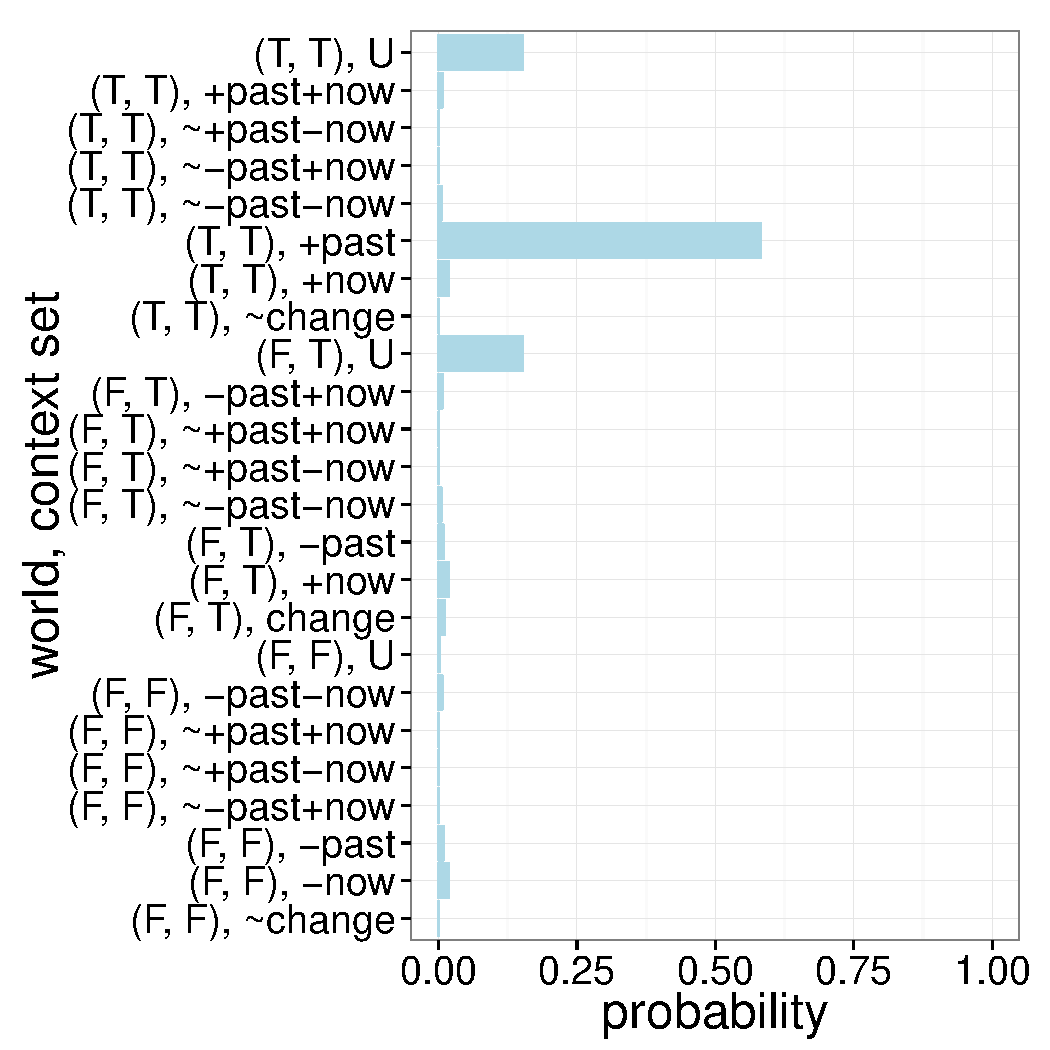
\includegraphics[scale=0.4]{figs/joint_CGprior_QUDnow.pdf}
 \caption{Pragmatic listener after hearing ``John did not stop smoking,'' with $\alpha=6$, CG prior + QUD$_\text{now}$\label{fig:joint-QUDnow}}
\vspace{-3ex}
\end{figure}

\noindent\textbf{Non-maximal QUDs} \quad
So far, we have been assuming that the QUD is maximal, i.e., the utterance 
 ``John did not stop smoking'' is chosen to address the question of
 whether John smoked in the past and whether John smokes now.
For this QUD, the RSA model with common ground prior predicts a tie between 
 $(T, T)$ with context set \verb=+past= and
 $(F, F)$ with context set \verb=-now=.
 
The maximal QUD is often assumed in applications of RSA models (though see \citeA{KaoEtAl2014-Cogsci}), but 
 in this case there are good reasons to consider non-maximal QUDs.
Empirically, as noted in the beginning, projection is sensitive to the QUD.
Theoretically, there has been a lot of discussion in the previous literature
 \cite{Beaver2010:Have-You-Noticed, SimonsEtAl2001:What-Projects-and-Why} on the relation between at-issueness and projection, where at-issueness is defined 
 relative to a QUD not necessarily maximal.
 
In our running example, Bob explicitly asked about whether John smokes, 
 which means that the QUD is presumably QUD$_\textrm{now}$ (i.e., ``Does John smoke?'').
When we use the previous RSA model with the common ground prior, but  
 replace QUD$_\textrm{max}$ with QUD$_\textrm{now}$ (summarized in the 
 last column of Table~\ref{tab:models}), the pragmatic listener's marginal distribution over worlds is shown in Figure~\ref{fig:RSA_QUDnow} and the joint
 distribution of world and context set is in Figure~\ref{fig:joint-QUDnow}.
We can see from Figure~\ref{fig:joint-QUDnow} that $(T, T)$ with context set
 \verb=+past= is 
 the only most likely outcome, and the world $(T, T)$ is the 
 only most likely world (and its probability increases with a higher $\alpha$).
This is exactly the projection pattern we aim to capture.

To understand why we obtain this result, we note that 
 when the QUD is QUD$_\textrm{now}$, $(F, F)$ with context set
 \verb=-now= is dispreferred because the context set \verb=-now= already entails 
 the answer to the QUD. 
That is, it is already known from the context set \verb=-now= that John does not 
 smoke now.
This means that the speaker would be maximally informative even if he says nothing.
As a result, the speaker would be unlikely to say ``John did not stop smoking'' 
 when the context set is \verb=-now=, and the pragmatic listener could therefore
 infer that the context set \verb=-now= is unlikely, which means that 
 $(T, T)$ with context set \verb=+past= is the only winner.

%The model's prediction changes when we use a different QUD. 
%When the QUD is whether John smoked in the past, the model predicts that 
% the listener will infer that world $(F, F)$ with common
% ground \verb=-now= is most likely, as shown in Fig.~\ref{fig:joint-QUDpast}.
%This means that John never smokes and the speaker takes for granted that 
% John does not smoke now.
%This type of projection might be accessible in a scenario where there
% is a rumor about John being a heavy smoker in the past, and the speaker uses 
% ``John did not stop smoking'' to jokingly refute it.

Hence the current model correctly predicts the projective behavior for 
 ``John did not stop smoking'' in the example scenario, where the QUD is explicitly
 given by Bob's question. 
Assuming that people generally care about information about now rather than 
 the past, i.e., the default or most salient QUD is QUD$_\text{now}$,
the model predicts that the preferred projective content of 
 ``John did not stop smoking'' without explicit QUD is that 
 John smoked in the past, which is also correct.

%This completes the RSA model. In the next section we will further illustrate its predictions about the interaction between projection and QUD. 

\

\noindent \textbf{Other QUDs} \quad 
We have introduced a RSA model with common ground and shown its
 predictions for QUD$_\textrm{now}$ and QUD$_\textrm{max}$.
The prediction is sensitive to the QUD---in Figure~\ref{fig:RSA_QUDs} we show predictions for eight different QUDs.
%In this section, we further explore the interaction between the QUD and projection
% predicted by the model. 
%Concretely, besides QUD$_\textrm{max}$, we consider all 7 QUDs with yes/no answers: 
% QUD$_\text{now}$, QUD$_\text{past}$, QUD$_\text{change}$,
% QUD$_\text{always}$, QUD$_\text{stop}$, QUD$_\text{start}$, and QUD$_\text{never}$.
%For instance, QUD$_\text{always}$ asks whether it is the case that John both smoked in
% the past and smokes now.
%The predictions of the RSA model for these QUDs are shown in
% Figure~\ref{fig:RSA_QUDs}.
In general, it seems that the model is making plausible predictions. 
For example, when the QUD is whether John has always smoked, ``John did not stop smoking'' implies that John has always smoked (Figure~\ref{fig:RSA_QUDalways}). 
When the QUD is whether John has never smoked, ``John did not stop smoking'' implies that John has never smoked (Figure~\ref{fig:RSA_QUDnever}). 
When the QUD is about whether John stopped smoking (Figure~\ref{fig:RSA_QUDstop}) 
 or there is a change (Figure~\ref{fig:RSA_QUDchange}), after hearing
 ``John did not stop smoking,'' the pragmatic listener still believes that that John 
 smoked in the past is roughly equally likely as that John did not smoke in the past. 
 (Compare this to Geurts' example, described earlier.)
Further experimental data will be needed to assess whether these predictions are borne out.



